\chapter{UJI COBA DAN EVALUASI}\label{chap:uji-coba-eval}

\tab Bab ini akan membahas terkait uji coba aplikasi yang telah dirancang dan diimplementasikan. Uji coba dilakukan untuk mengetahui kinerja aplikasi dengan lingkungan uji coba yang telah ditentukan.

\section{Lingkungan Uji Coba}
\tab Lingkungan yang digunakan untuk pengujian meliputi perangkat keras dan
perangkat lunak yang dijelaskan sebagai berikut.

\begin{enumerate}
	\item Perangkat Keras:
	\begin{itemize}
		\item Prosesor 2.6 GHz Intel Core i5 (I5-4278U)
		\item Memori 8 GB 1600 MHz DDR3
	\end{itemize}
	\item Perangkat Lunak:
	\begin{itemize}
		\item Sistem operasi macOS Mojave Versi 10.14.5
		\item Bahasa Pemrograman Python 3.7.3
	\end{itemize}			
\end{enumerate}

\section{Data Uji Coba}

\tab Terdapat tiga jenis data yang akan digunakan dalam pengujian Tugas Akhir ini. Tiga jenis data tersebut terdiri dari data \textit{independent} (IND), data \textit{anti-correlated} (ANT), dan data \textit{Forest-Covertype} (FC).

\subsection{Data \textit{Independent} (IND)}
\tab Data \textit{independent} (IND) adalah himpunan data yang memiliki persebaran nilai atribut yang acak dan tidak saling terpengaruh satu sama lain. Data ini adalah data sintetis yang dibuat untuk menguji performa algoritma jika berhadapan dengan data yang nilai atributnya tidak memiliki keterkaitan satu sama lain. Rentang nilai yang digunakan untuk setiap atribut adalah 1 – 200.

\subsection{Data \textit{Anti-Correlated} (ANT)}
\tab Data \textit{anti-correlated} (ANT) adalah himpunan data yang memiliki
persebaran nilai atribut yang saling bertolak belakang antara satu
atribut dengan atribut lainnya, artinya sebuah data memiliki
nilai yang sangat baik pada salah satu atributnya, namun sangat
buruk pada atribut lainnya. Data ini adalah data sintetis yang dibuat untuk menguji performa algoritma jika berhadapan dengan data yang memiliki banyak titik skyline. Rentang nilai yang digunakan untuk setiap
atribut adalah 1 – 200.

\subsection{Data \textit{Forest Cover Type} (FC)}
\tab Data \textit{Forest Cover Type} (FC) adalah himpunan data asli yang berisi hasil pengamatan pohon dari empat area Hutan Nasional Roosevelt di Colorado. Semua pengamatan adalah variabel kartografi dari 30 meter x 30 meter bagian hutan. Dataset ini mencakup informasi tentang jenis pohon, jangkauan bayangan, jarak ke \textit{landmark} terdekat (jalan dan sebagainya), jenis tanah, dan topografi lokal. \textit{Dataset} ini adalah bagian dari \textit{UCI Machine Learning Repository} yang dikumpulkan oleh Blackard, Dean, dan Anderson di Colorado \textit{State University} \cite{fc}.

Himpunan data \textit{Forest Cover Type} (FC) terdiri dari 581.012 data dan memiliki 55 dimensi atribut. Tidak ditemukan nilai yang hilang atau anomali
pada himpunan data ini. Seluruh atribut bertipe data numerik
dengan rincian dapat dilihat pada Tabel \ref{tab:atribut-fc}.

\begin{table}[H]
	\centering
	\begin{tabular}{ | p{6cm} | p{1cm} | }
		\hline
		\multicolumn{1}{|c}{\textbf{Nama Kolom}} & \multicolumn{1}{|c|}{\textbf{Jumlah Kolom}} \\ \hline \hline
		Elevation & 1 \\ \hline
		Aspect & 1 \\ \hline
		Slope & 1  \\ \hline
		Horizontal\_Distance\_To\_Hydrology & 1 \\ \hline 
		Vertical\_Distance\_To\_Hydrology & 1 \\ \hline 
		Horizontal\_Distance\_To\_Roadways & 1 \\ \hline
		Hillshade\_9am & 1 \\ \hline
		Hillshade\_Noon & 1 \\ \hline
		Hillshade\_3pm & 1 \\ \hline
		Horizontal\_Distance\_To\_Fire\_Points & 1 \\ \hline
		Wilderness\_Area & 4 \\ \hline
		Soil\_Type & 40 \\ \hline
		Cover\_Type & 1 \\ \hline
	\end{tabular} \caption{Atribut pada Himpunan Data \textit{Forest Cover Type}}
	\label{tab:atribut-fc}
\end{table}

Data \textit{Forest Cover Type} (FC) adalah himpunan data yang
diambil dari sumber sebenarnya. Penggunaan data ini bertujuan
untuk menguji performa algoritma pada data dengan persebaran
dan rentang nilai atribut sebenarnya yang bersifat saling berkaitan.

\section{Skenario Uji Coba} \label{skenarioujicoba}
\tab Uji coba ini dilakukan untuk menguji apakah program yang telah diimplementasikan dapat berjalan dengan sebagaimana mestinya. Uji coba akan dibagi menjadi dua jenis, yaitu uji coba fungsionalitas dan uji coba performa.

\subsection{Uji Coba Fungsionalitas}
\tab Skenario uji coba fungsionalitas berfokus pada pengujian apakah aplikasi dapat digunakan sesuai dengan kebutuhan fungsional pada Tabel \ref{tab:kebutuhan-fungsional}. Skenario pengujian fungsionalitas aplikasi ditunjukkan pada Tabel \ref{tab:uji-coba-fungsional}.

\begin{table}[H]
	\centering
	\begin{tabular}{ | c | p{8cm} | }
		\hline
		\multicolumn{1}{|c}{\textbf{No.}} & \multicolumn{1}{|c|}{\textbf{Deskripsi Kebutuhan}} \\ \hline \hline
		1 & Pengguna dapat mengunggah data \\ \hline
		2 & Pengguna dapat melihat informasi dan pratinjau data \\ \hline
		3 & Pengguna dapat melihat visualisasi data  \\ \hline
		4 & Pengguna dapat memilih algoritme yang digunakan untuk \textit{data precomputing}\\ \hline
		5 & Pengguna dapat memasukkan kueri pencarian \\ \hline
		6 & Pengguna dapat melihat hasil kueri \\ \hline
	\end{tabular} \caption{Skenario Uji Coba Fungsionalitas}
	\label{tab:uji-coba-fungsional}
\end{table}

\subsection{Uji Coba Performa}
\tab Pengujian performa bertujuan untuk membandingkan kinerja masing-masing algoritme dalam melakukan \textit{data precomputing}. Dalam sebuah percobaan atau pengujian, biasanya dikenal adanya tiga jenis variabel, yaitu variabel kontrol, manipulasi, dan respon. 

Variabel kontrol adalah variabel yang dikendalikan, biasanya dibuat konstan sehingga pengaruh variabel manipulasi terhadap variabel respon tidak dipengaruhi oleh faktor luar yang tidak diteliti. Variabel manipulasi adalah variabel yang dapat memicu suatu perubahan bagi variabel respon. Variabel respon adalah variabel yang berubah akibat dari variabel manipulasi.

Dalam pengujian ini, variabel kontrol yang digunakan adalah jenis data dan jenis algoritme, variabel manipulasinya adalah jumlah data dan jumlah dimensi data, sedangkan variabel responnya berupa waktu eksekusi dan penggunaan memori. Skenario pengujian performa ditunjukkan pada Tabel \ref{tab:uji-coba-performa-precompute}.

\begin{longtable}{| c | p{3cm} | p{1cm} | p{2.5cm} | p{1.5cm} |}
	\caption{Skenario Uji Coba Performa \textit{Data Precomputing} \label{tab:uji-coba-performa-precompute}}\\
	\hline
	\textbf{No.} & \textbf{Jenis Algoritme} & \textbf{Jenis Data} & \textbf{Jumlah Data ($n$)} & \textbf{Jumlah Dimensi ($d$)} \\ \hline
	\endfirsthead
	\hline
	\textbf{No.} & \textbf{Jenis Algoritme} & \textbf{Jenis Data} & \textbf{Jumlah Data ($n$)} & \textbf{Jumlah Dimensi ($d$)} \\ \hline
	\endhead
	\multirow{3}{*}{1} & k-MPPTI & \multirow{3}{1cm}{IND} & \multirow{3}{2.5cm}{100, 500, 1000, 5000, 10000} & \multirow{3}{1.5cm}{3} \\ \cline{2-2} \nopagebreak
	& k-MPPTI RSL & & & \\ \cline{2-2} \nopagebreak
	& k-MPPTI Paralel & & & \\ \hline
	\multirow{3}{*}{2} & k-MPPTI & \multirow{3}{1cm}{ANT} & \multirow{3}{2.5cm}{100, 500, 1000, 5000, 10000} & \multirow{3}{1.5cm}{3}\\ \cline{2-2} \nopagebreak
	& k-MPPTI RSL & & & \\ \cline{2-2} \nopagebreak
	& k-MPPTI Paralel & & & \\ \hline
	\multirow{3}{*}{3} & k-MPPTI & \multirow{3}{1cm}{FC} & \multirow{3}{2.5cm}{100, 500, 1000, 5000, 10000} & \multirow{3}{1.5cm}{3}\\ \cline{2-2} \nopagebreak
	& k-MPPTI RSL & & & \\ \cline{2-2} \nopagebreak
	& k-MPPTI Paralel & & & \\ \hline 
	\multirow{3}{*}{4} & k-MPPTI & \multirow{3}{1cm}{IND} & \multirow{3}{2.5cm}{1000} & \multirow{3}{1.5cm}{2, 3, 5, 7, 10}\\ \cline{2-2}	\nopagebreak	
	& k-MPPTI RSL & & & \\ \cline{2-2} \nopagebreak
	& k-MPPTI Paralel & & & \\ \hline
	\multirow{3}{*}{5} & k-MPPTI & \multirow{3}{1cm}{ANT} & \multirow{3}{2.5cm}{1000} & \multirow{3}{1.5cm}{2, 3, 5, 7, 10}\\ \cline{2-2}\nopagebreak
	& k-MPPTI RSL & & & \\ \cline{2-2} \nopagebreak
	& k-MPPTI Paralel & & & \\ \hline
	\multirow{3}{*}{6} & k-MPPTI & \multirow{3}{1cm}{FC} & \multirow{3}{2.5cm}{1000} & \multirow{3}{1.5cm}{2, 3, 5, 7, 10}\\ \cline{2-2} \nopagebreak
	& k-MPPTI RSL & & & \\ \cline{2-2} \nopagebreak
	& k-MPPTI Paralel & & & \\ \hline
\end{longtable}

\section{Analisis Hasil Uji Coba}
\tab Setelah pengujian dilakukan, selanjutnya adalah menganalisis hasil uji coba. Analisis hasil uji coba dibagi menjadi dua bagian, yaitu hasil uji coba fungsionalitas dan hasil uji coba performa.

\subsection{Uji Coba Fungsionalitas}
\tab Pengujian fungsionalitas dilakukan sesuai dengan skenario daftar kebutuhan fungsional pada Tabel \ref{tab:uji-coba-fungsional} yang hasilnya dapat dilihat pada tabel berikut. 

\begin{table}[H]
	\centering
	\begin{tabular}{ | c | p{5cm} | p{2cm} | }
		\hline
		\multicolumn{1}{|c}{\textbf{No.}} & \multicolumn{1}{|c}{\textbf{Deskripsi Kebutuhan}} & \multicolumn{1}{|c|}{\textbf{Hasil}}\\ \hline \hline
		1 & Pengguna dapat mengunggah data & Berhasil\\ \hline
		2 & Pengguna dapat melihat informasi dan pratinjau data & Berhasil\\ \hline
		3 & Pengguna dapat melihat visualisasi data & Berhasil \\ \hline
		4 & Pengguna dapat memilih algoritme yang digunakan untuk \textit{data precomputing} & Berhasil\\ \hline
		5 & Pengguna dapat memasukkan kueri pencarian & Berhasil \\ \hline
		6 & Pengguna dapat melihat hasil kueri & Berhasil\\ \hline
	\end{tabular} \caption{Hasil Uji Coba Fungsionalitas}
	\label{tab:hasil-uji-coba-fungsional}
\end{table}

\pagebreak
Berdasarkan hasil uji coba, aplikasi dapat memenuhi semua kebutuhan fungsional, yakni mengunggah data (Gambar \ref{fig:hasil-performa1}), melihat informasi (Gambar \ref{fig:hasil-performa3}) dan pratinjau data (Gambar \ref{fig:hasil-performa4}), melihat visualisasi data dalam bentuk lini masa (Gambar \ref{fig:hasil-performa5}), memilih algoritme untuk \textit{data precomputing} (Gambar \ref{fig:hasil-performa1}), memasukkan kueri pencarian (Gambar \ref{fig:hasil-performa6}), dan melihat hasil kueri (Gambar \ref{fig:hasil-performa6}).

Sebagai tambahan, aplikasi juga memiliki fitur \textit{session} (Gambar \ref{fig:hasil-performa7}) supaya pengguna dapat melakukan dua kali proses \textit{data precomputing} menggunakan data yang berbeda tanpa saling menumpuk satu sama lain. Pengguna hanya perlu memilih \textit{session} yang diinginkan, kemudian melakukan kueri pencarian atau melihat visualisasi data. \\

\begin{figure}[H]
	\centering
	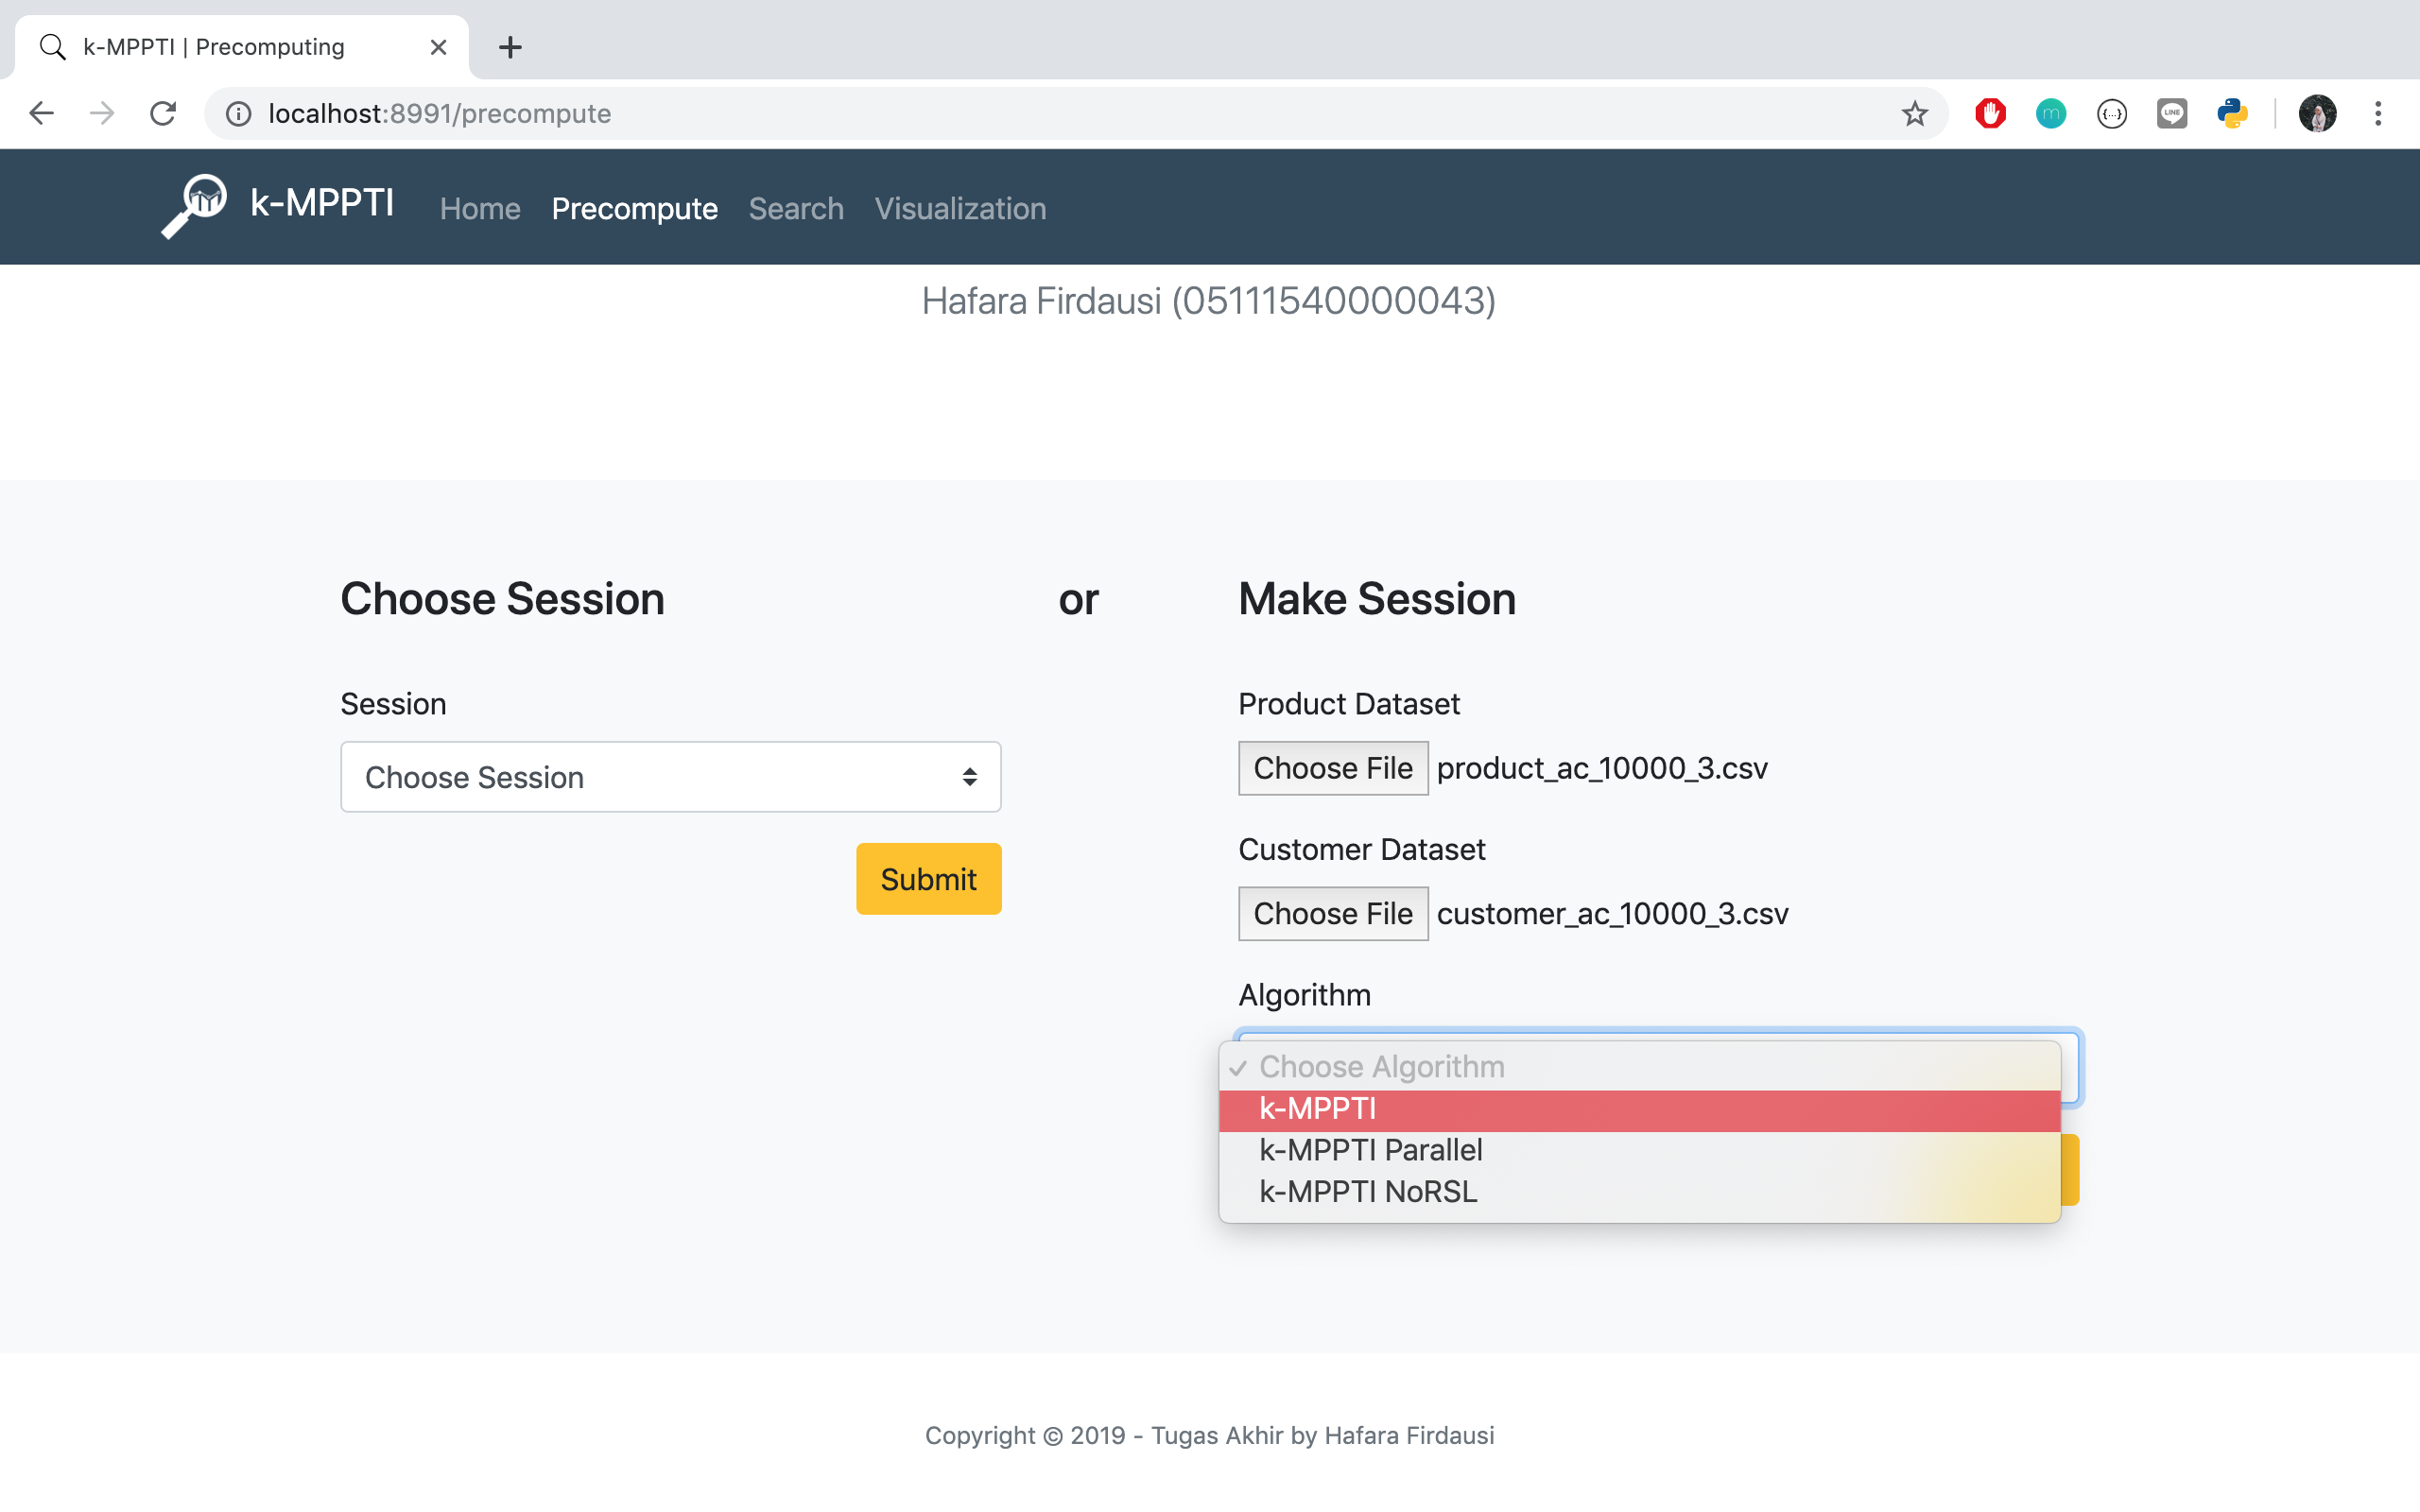
\includegraphics[width=9cm]{assets/img/bab5/hasil2.png}
	\caption{Hasil Uji Coba: Mengunggah Data dan Memilih Algoritme \textit{Data Precomputing}}
	\label{fig:hasil-performa1}
\end{figure}

\begin{figure}[H]
	\centering
	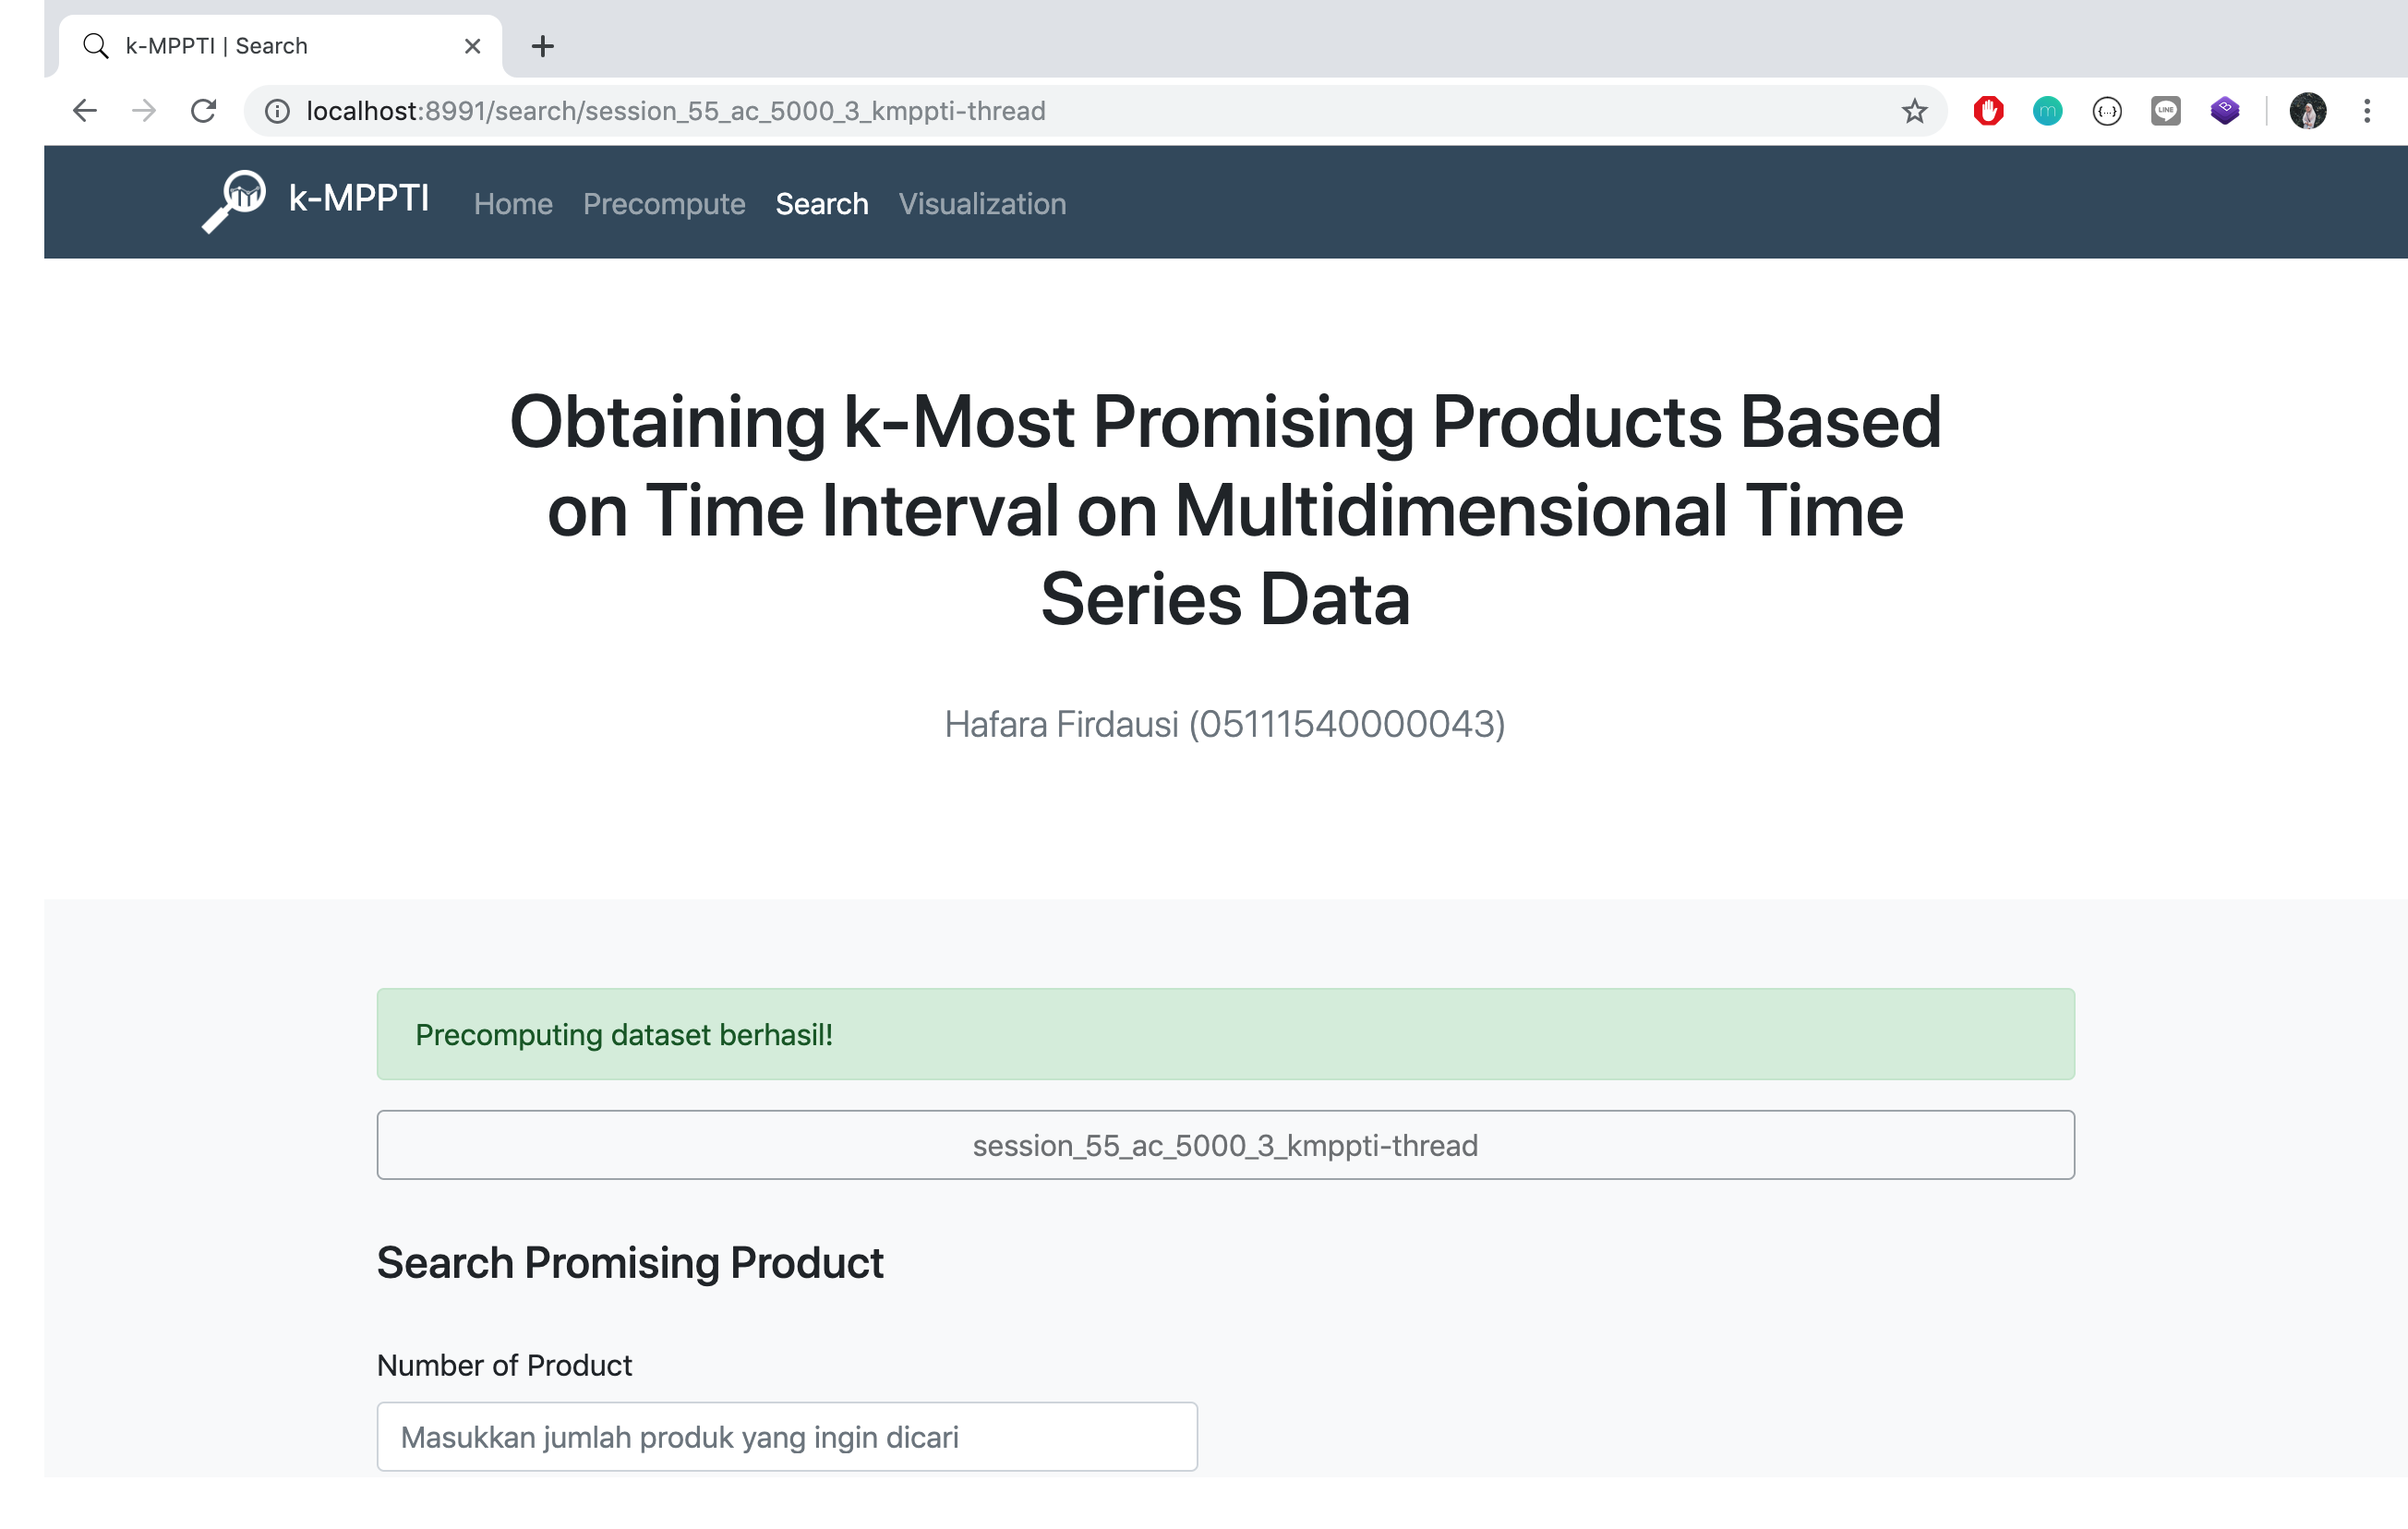
\includegraphics[width=9cm]{assets/img/bab5/hasil1.png}
	\caption{Hasil Uji Coba: \textit{Data Precomputing} Berhasil}
	\label{fig:hasil-performa2}
\end{figure}

\begin{figure}[H]
	\centering
	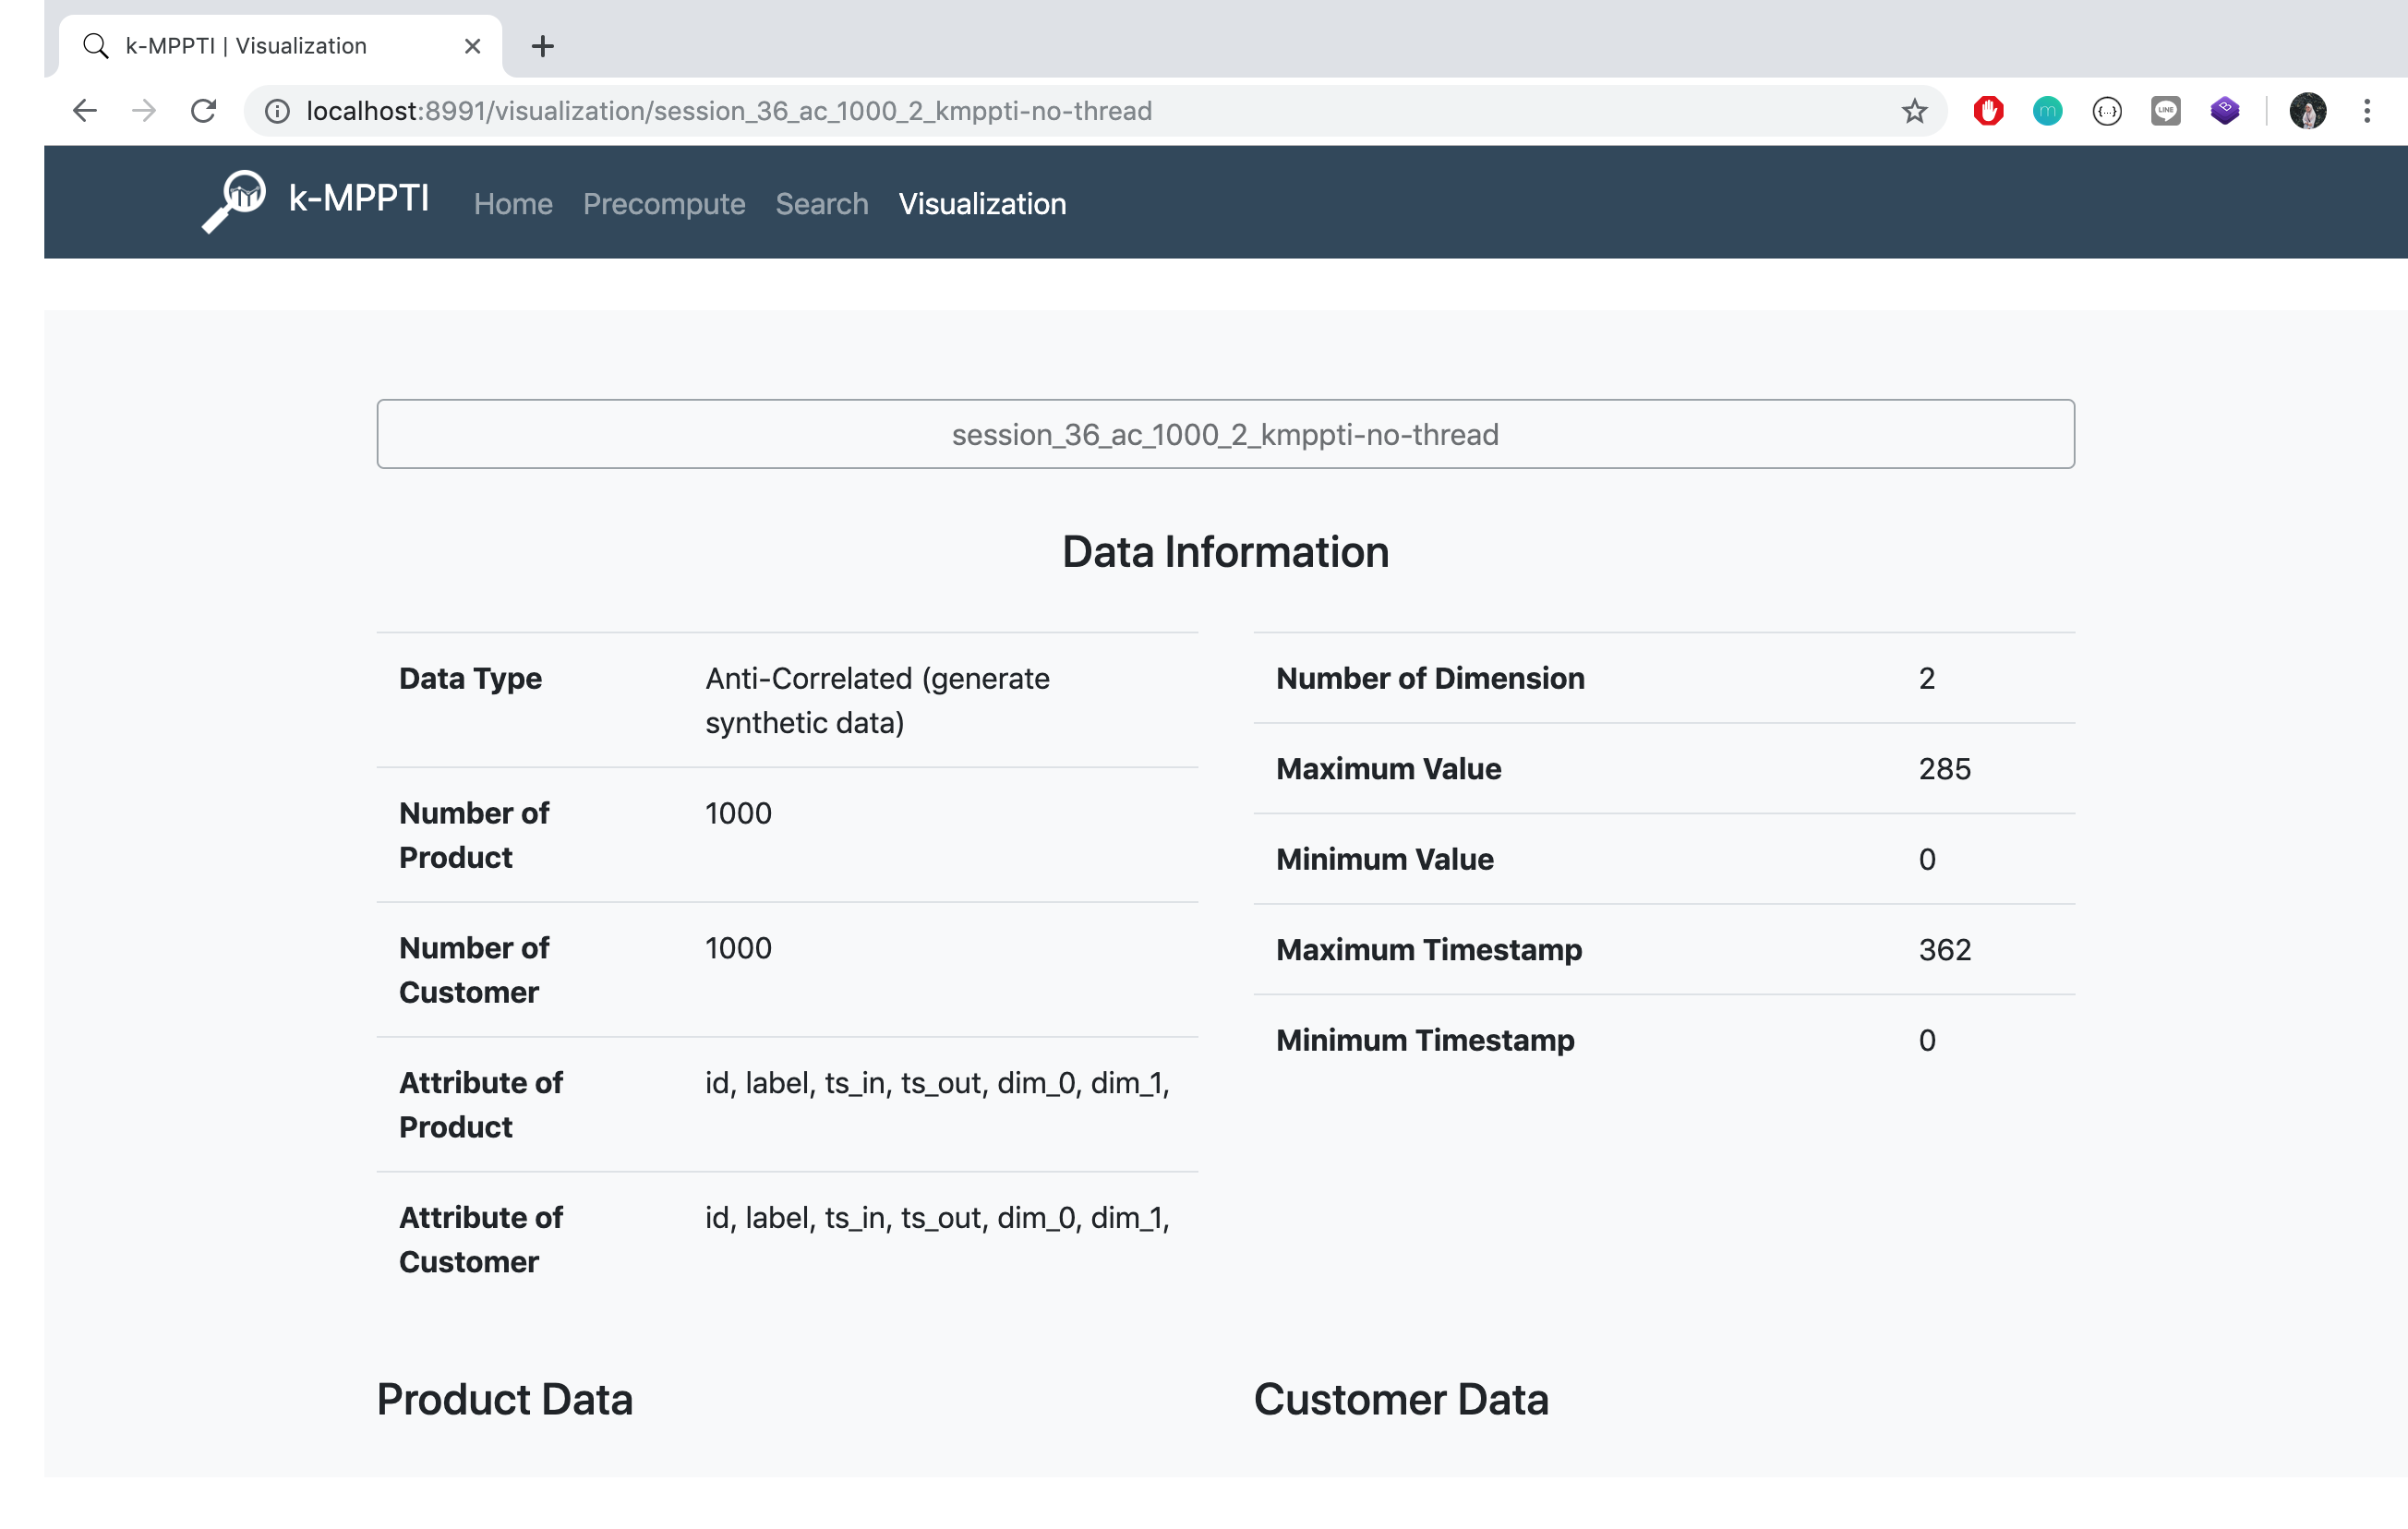
\includegraphics[width=9cm]{assets/img/bab5/hasil3.png}
	\caption{Hasil Uji Coba: Melihat Informasi Data}
	\label{fig:hasil-performa3}
\end{figure}

\begin{figure}[H]
	\centering
	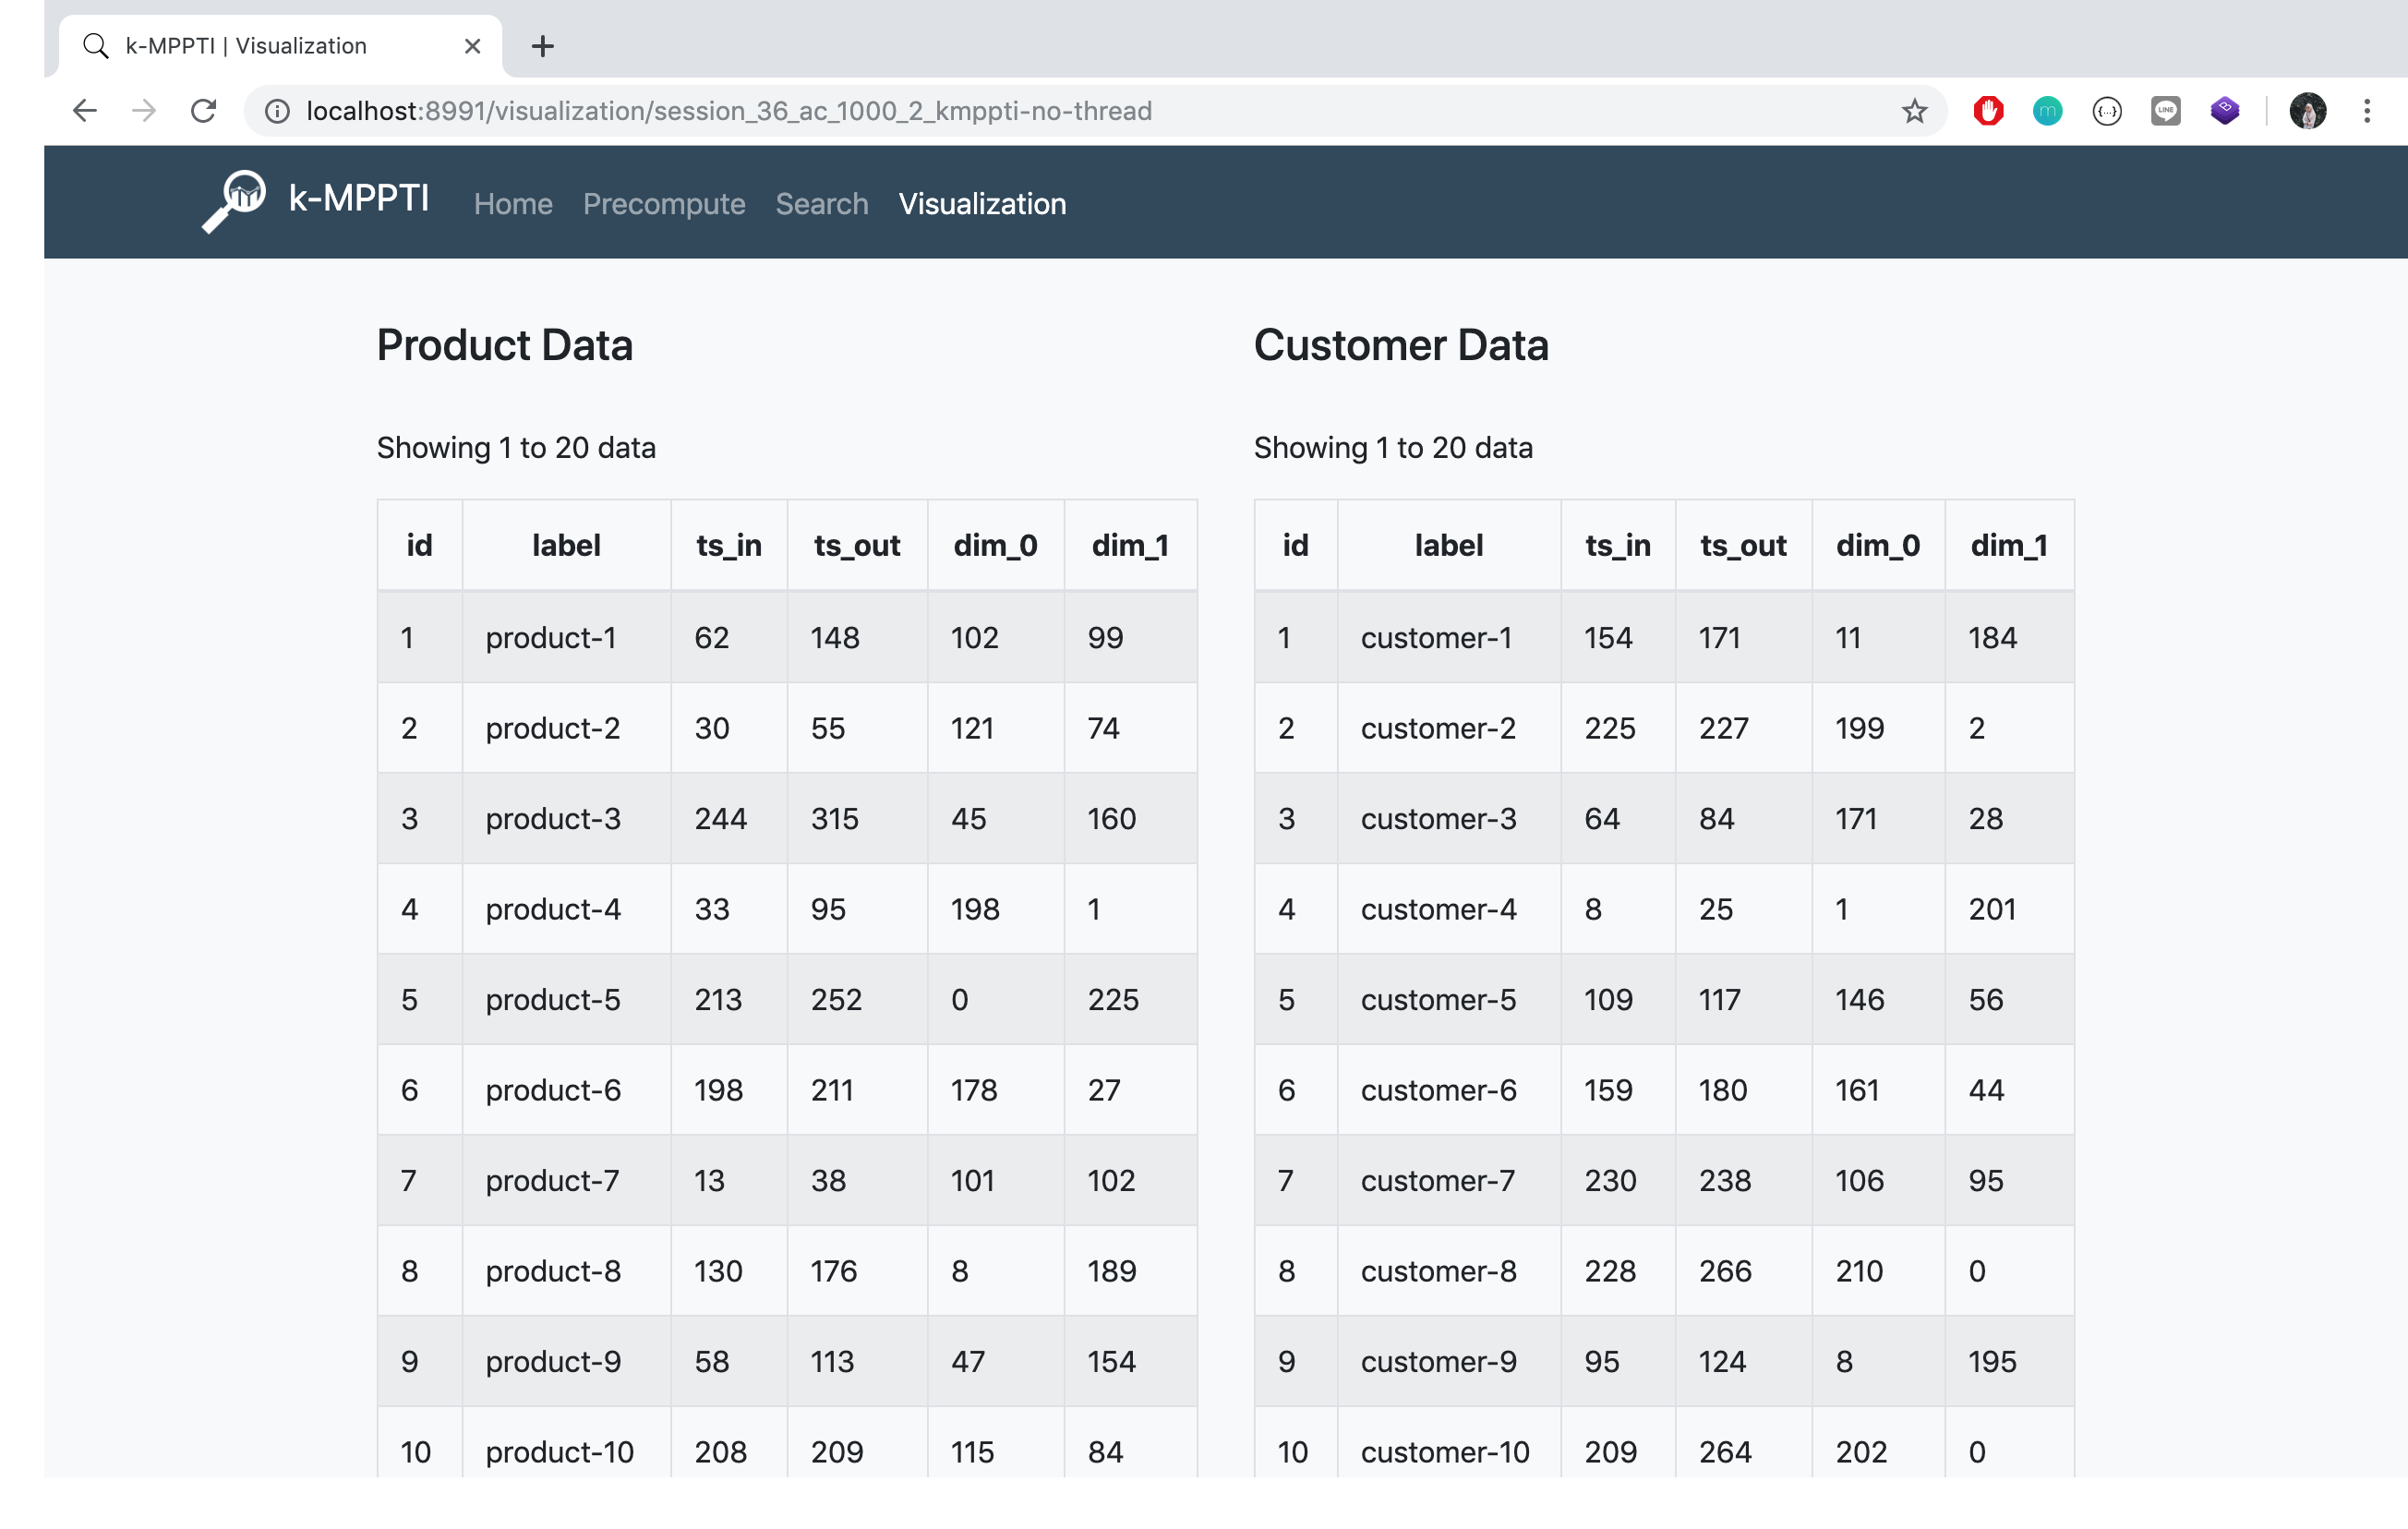
\includegraphics[width=9cm]{assets/img/bab5/hasil4.png}
	\caption{Hasil Uji Coba: Melihat Pratinjau Data Berupa Tabel}
	\label{fig:hasil-performa4}
\end{figure}

\begin{figure}[H]
	\centering
	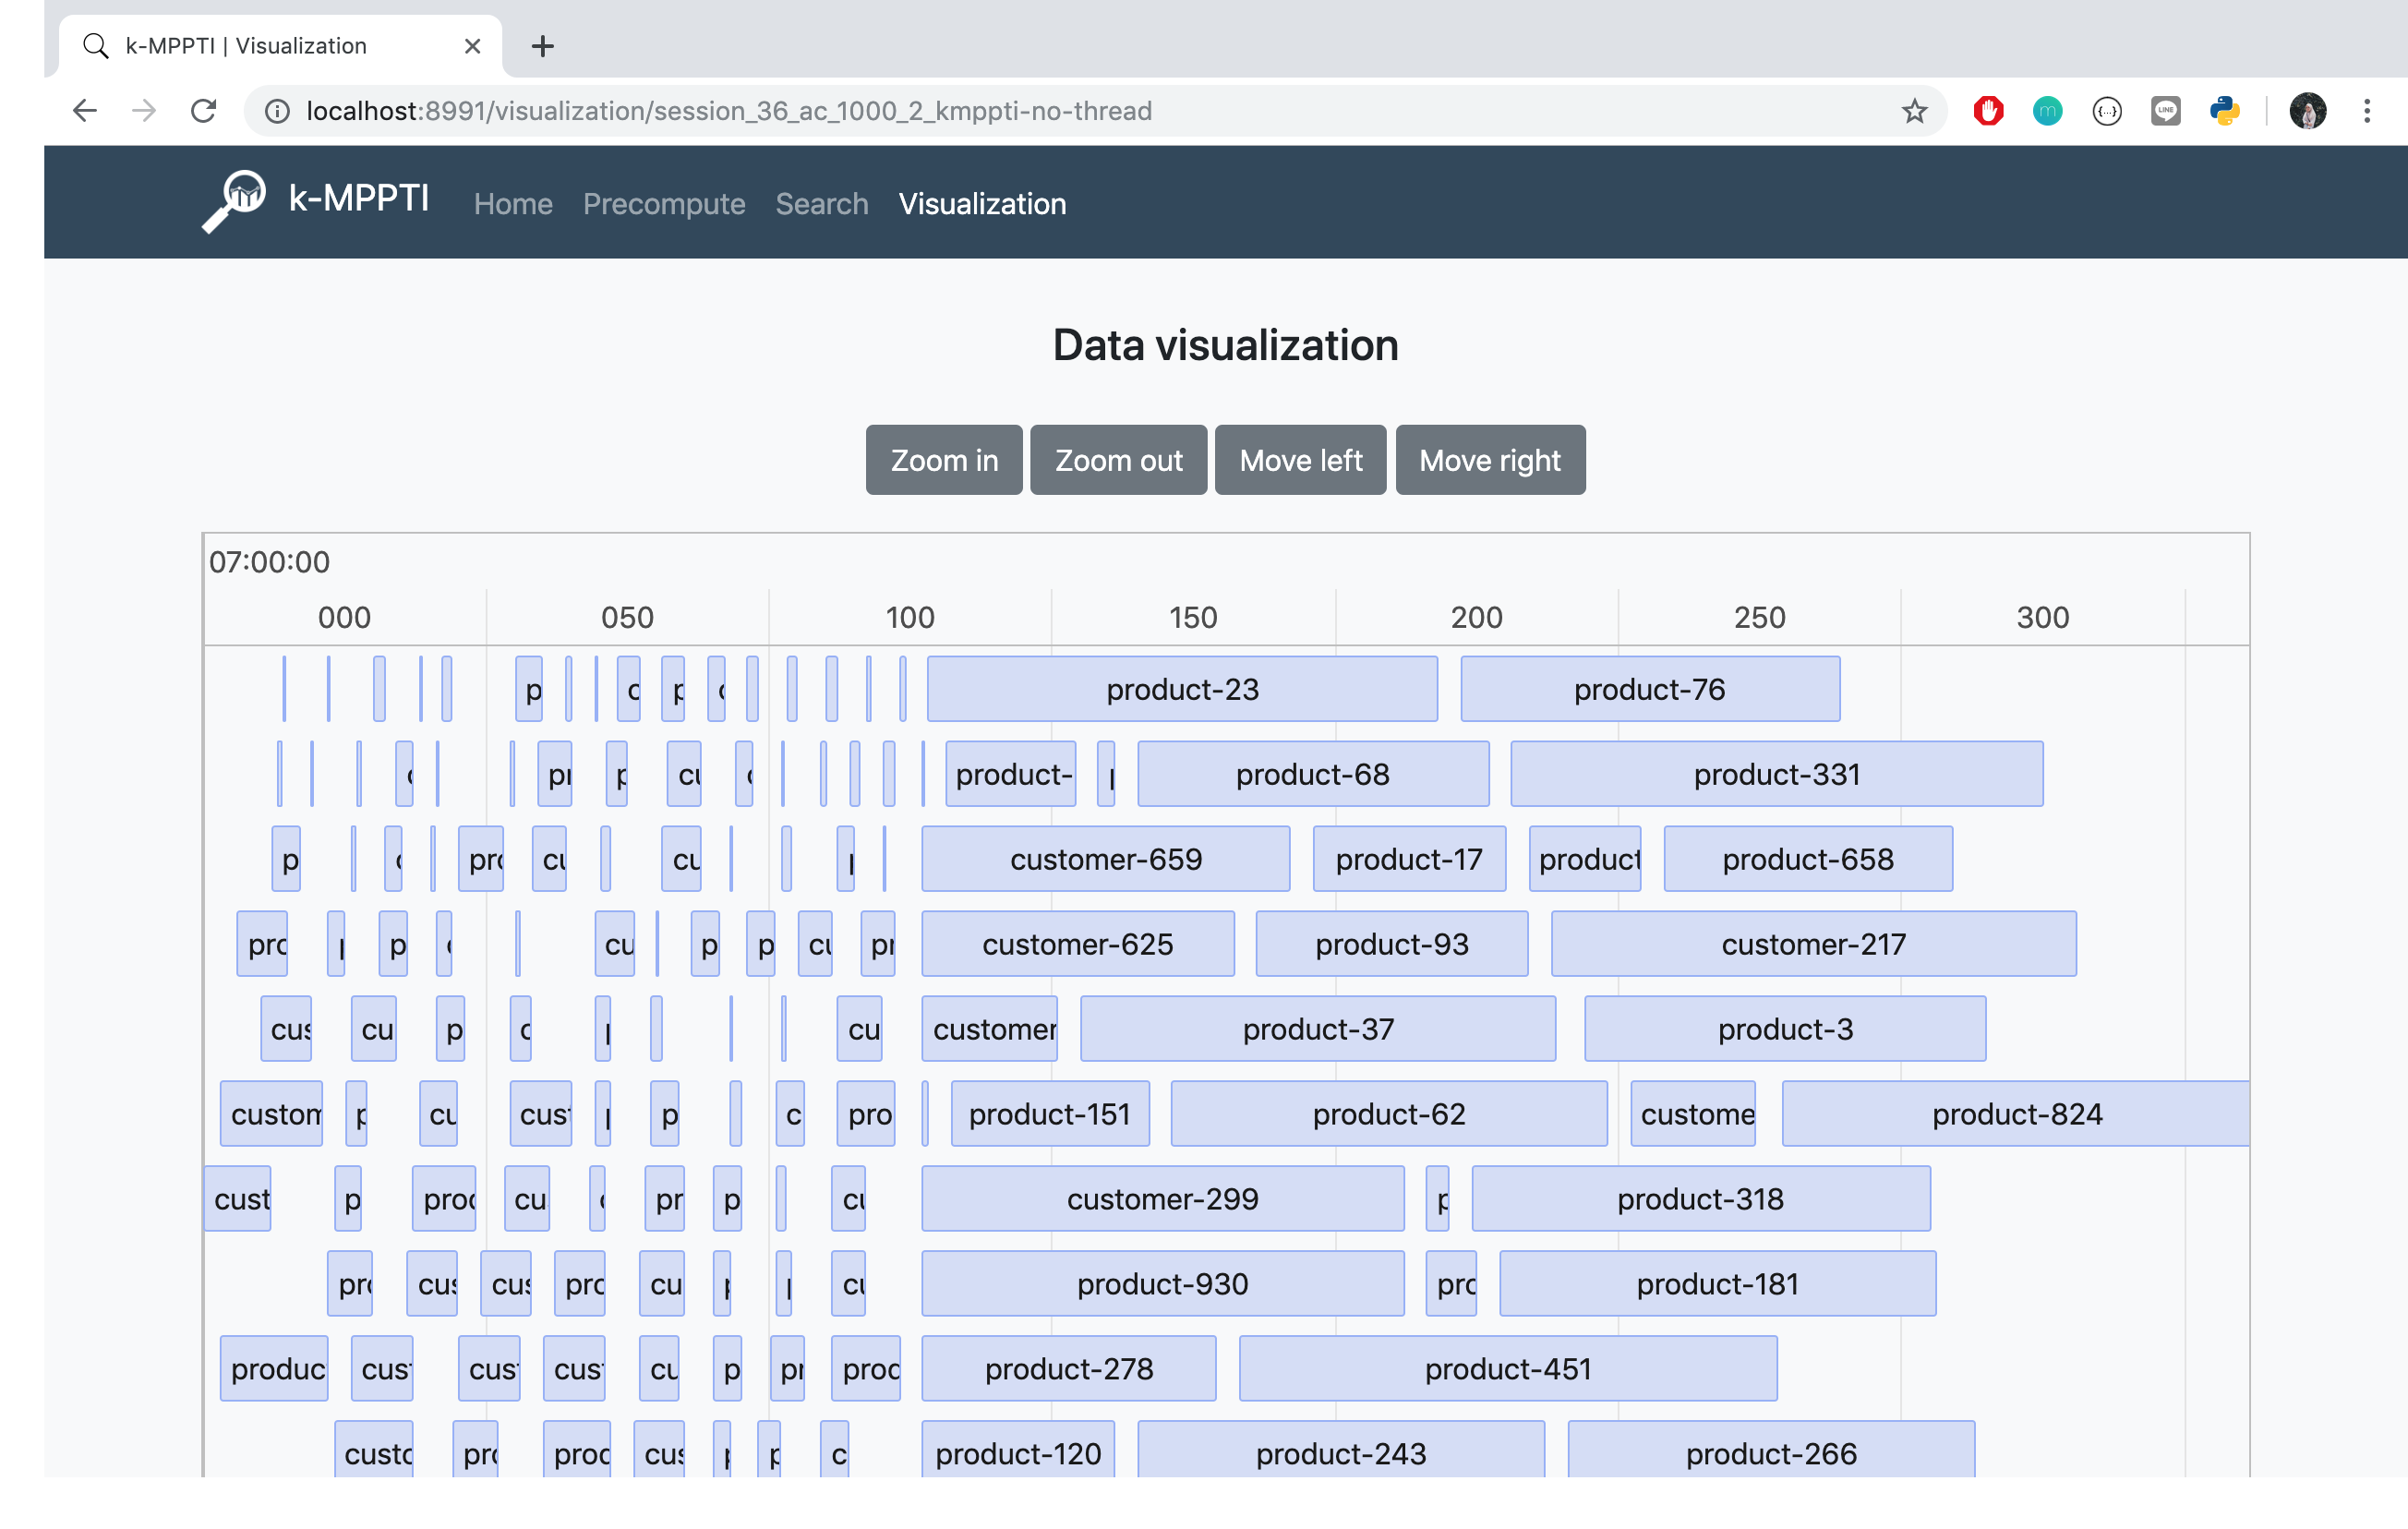
\includegraphics[width=9cm]{assets/img/bab5/hasil5.png}
	\caption{Hasil Uji Coba: Melihat Visualisasi Data Berupa Lini Masa}
	\label{fig:hasil-performa5}
\end{figure}

\begin{figure}[H]
	\centering
	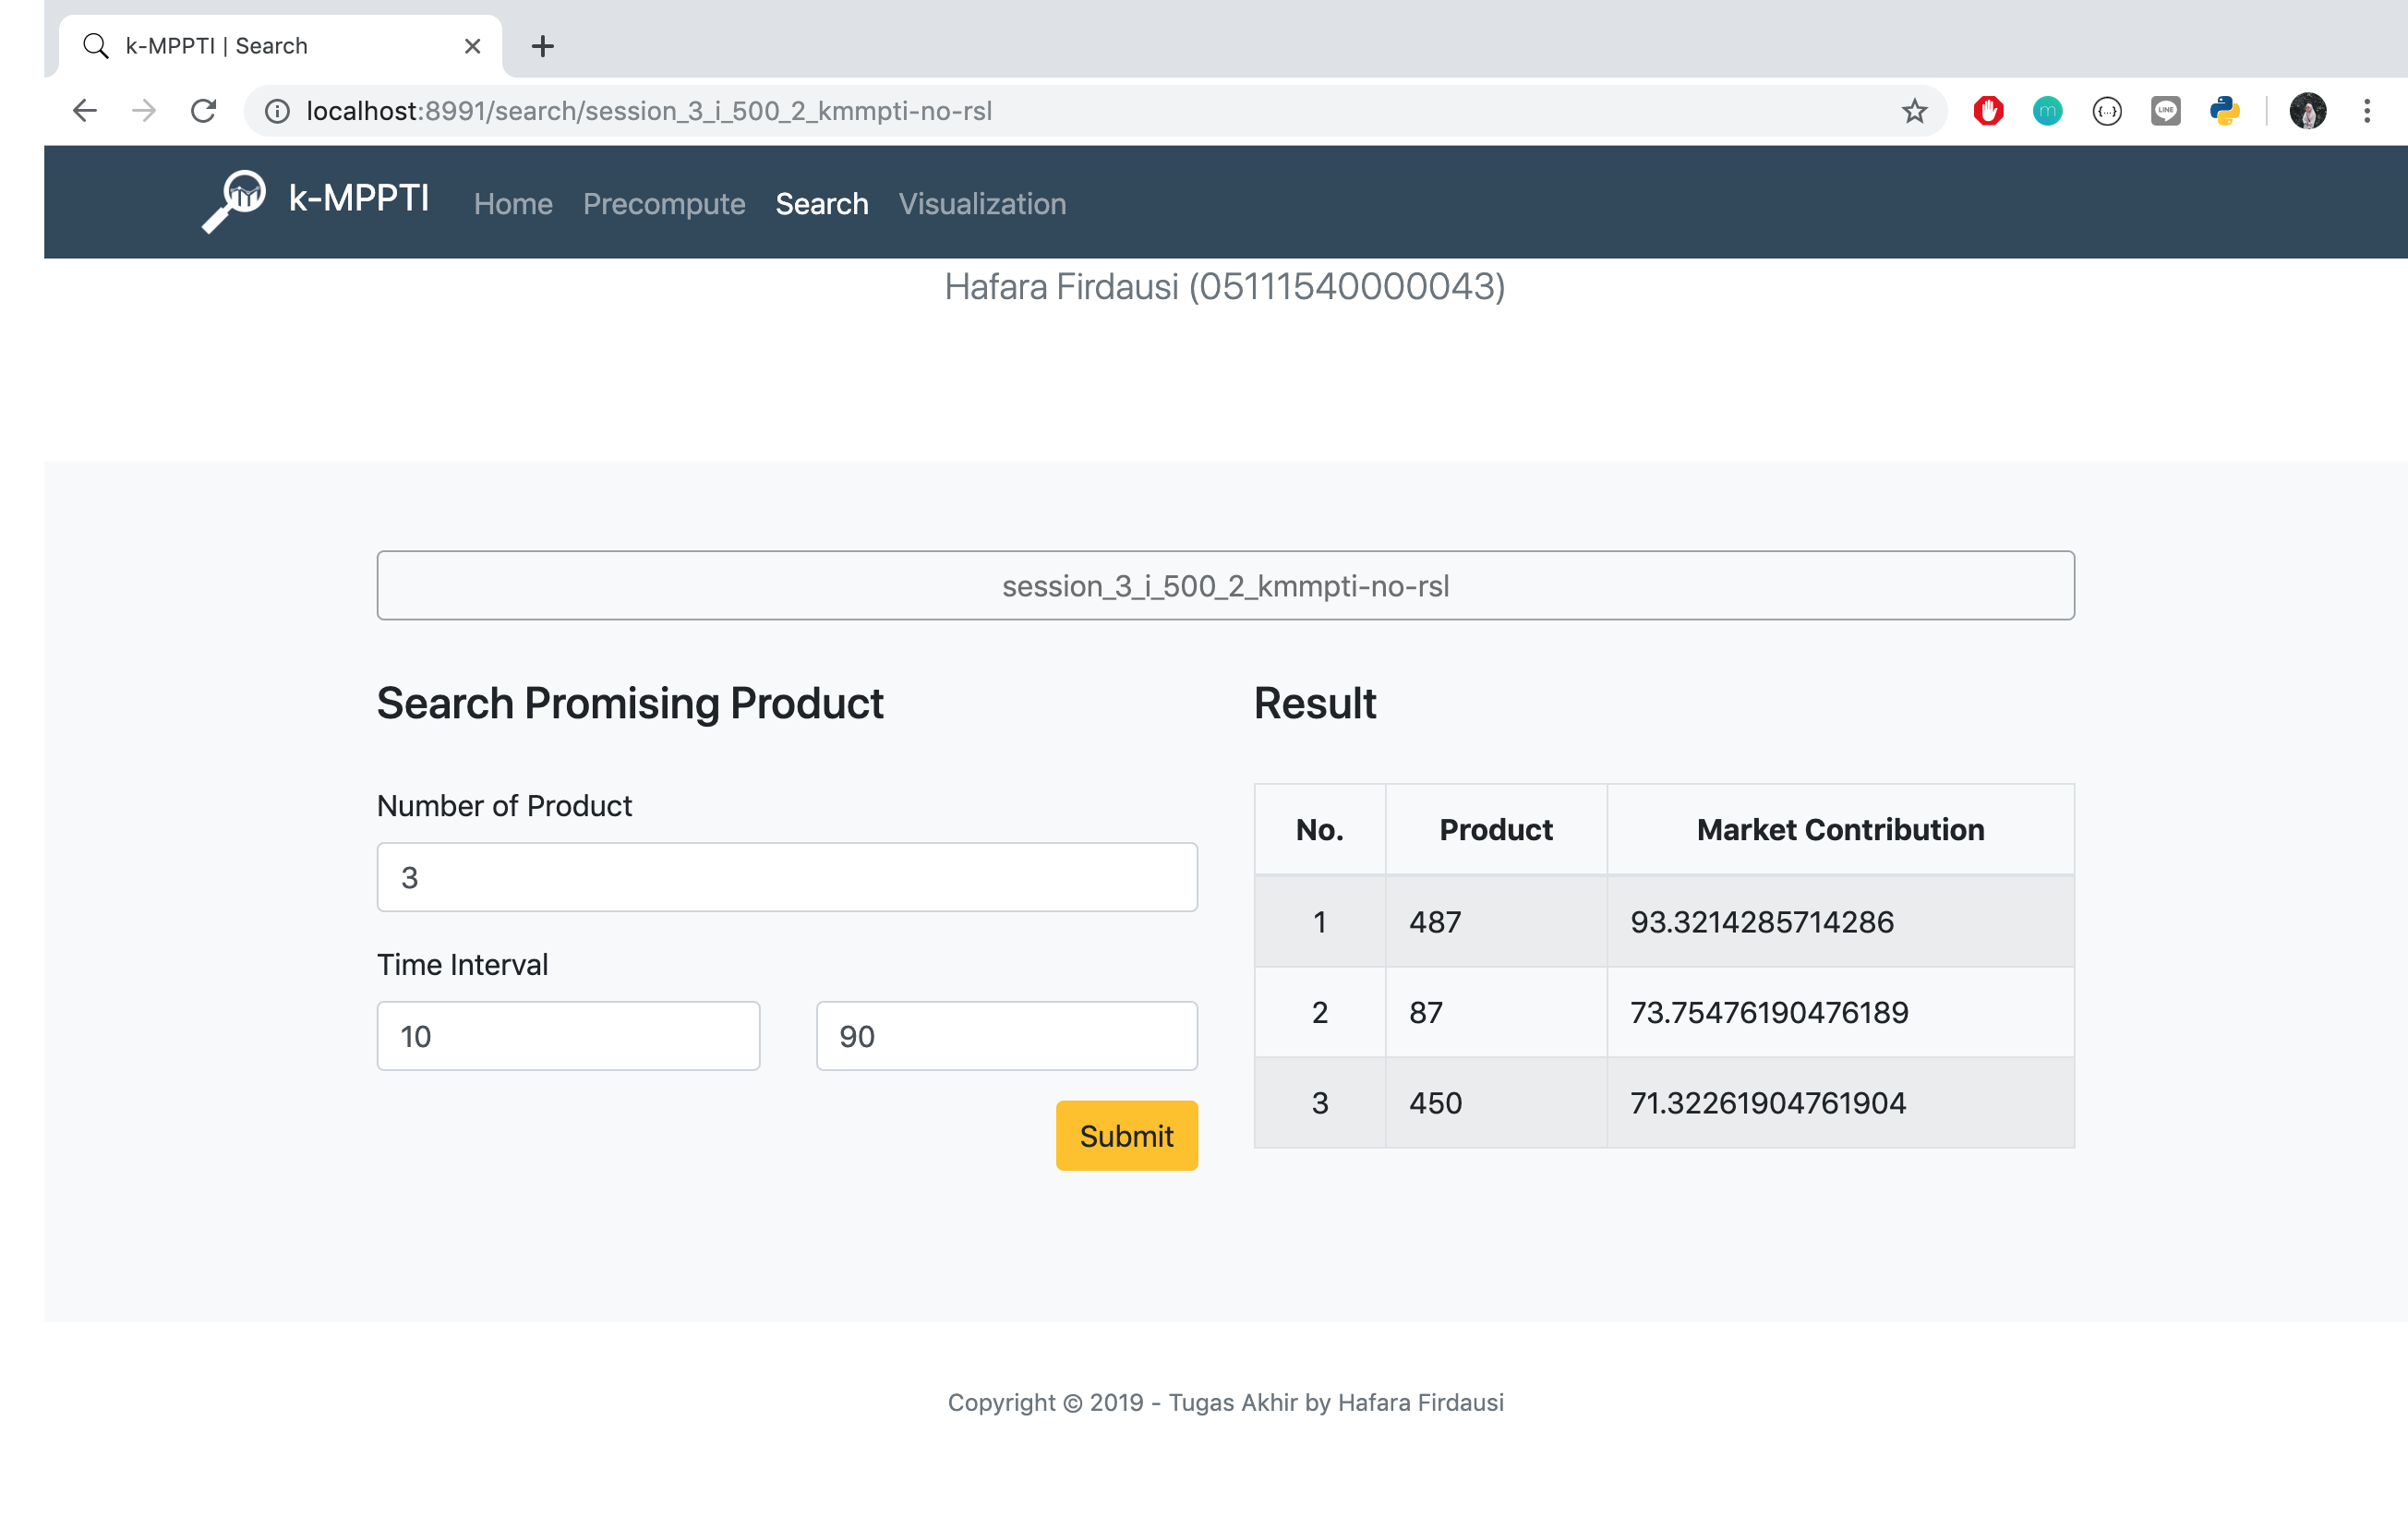
\includegraphics[width=9cm]{assets/img/bab5/hasil6.png}
	\caption{Hasil Uji Coba: Memasukkan Kueri Pencarian dan Melihat Hasil Kueri}
	\label{fig:hasil-performa6}
\end{figure}

\begin{figure}[H]
	\centering
	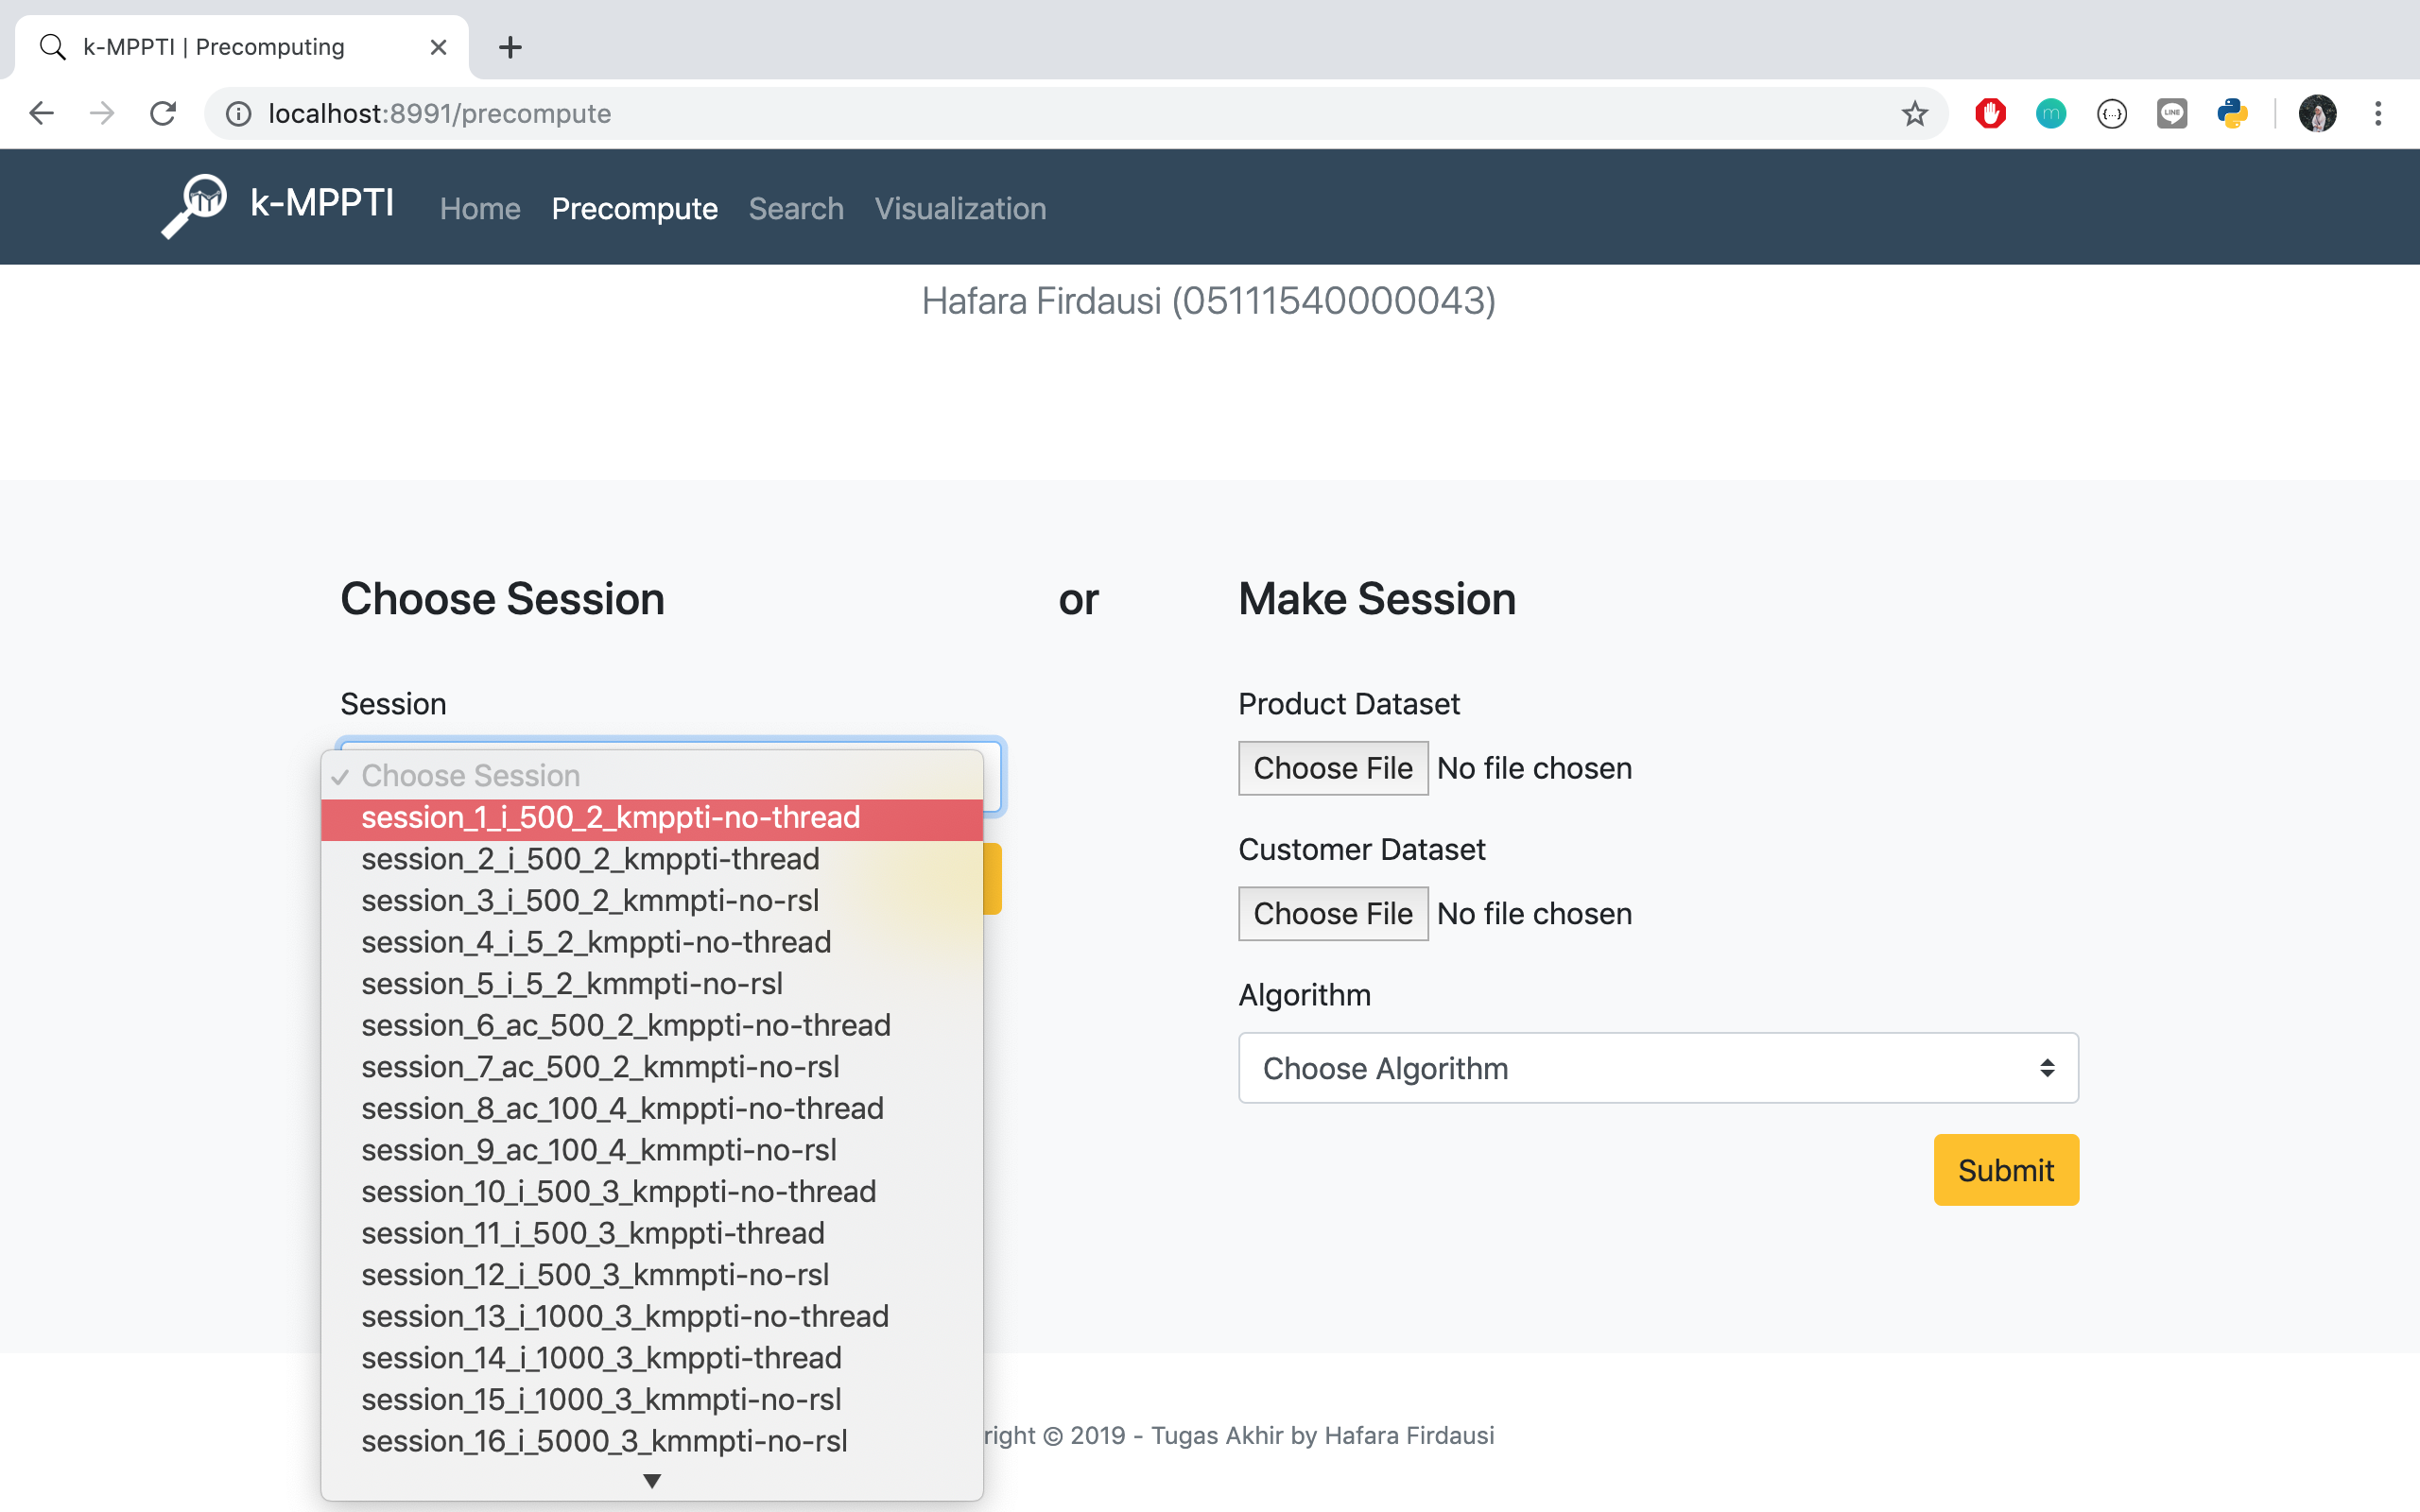
\includegraphics[width=9cm]{assets/img/bab5/hasil7.png}
	\caption{Hasil Uji Coba: Memilih \textit{Session}}
	\label{fig:hasil-performa7}
\end{figure}

\subsection{Uji Coba Performa}
\subsubsection{Pengaruh Jumlah Data Terhadap Performa Algoritme}

\subsubsection{Pengaruh Jumlah Dimensi Terhadap Performa Algoritme}